\section{t-SNE}
\begin{frame}{t-SNE: Why Do We Need It?}

\textbf{PCA is great... but it's linear.} Many datasets have \textbf{non-linear} structure.

\vspace{0.8em}
\begin{columns}[c]
\begin{column}{1.0\textwidth}
\begin{tcolorbox}[colback=blue!5, colframe=blue!50, title=\textbf{Problem}]
\begin{itemize}
\item High-dimensional data can be hard to visualize
\item PCA may \textbf{mix} classes if the separation is non-linear
\item We mainly want a \textbf{good 2D plot} for exploration
\end{itemize}
\end{tcolorbox}
\end{column}
\end{columns}

\end{frame}


% --- SLIDE: t-SNE intuition (no math) ---
\begin{frame}{t-Distributed Stochastic Neighbor Embedding (t-SNE)}

\begin{tcolorbox}[colback=yellow!8, colframe=orange!60, title=\textbf{Main Idea}]
t-SNE tries to build a 2D map where:
neighbors in high-D remain neighbors in 2D.
\end{tcolorbox}

\vspace{0.8em}
\begin{columns}[c]

\begin{column}{1.0\textwidth}
\centering
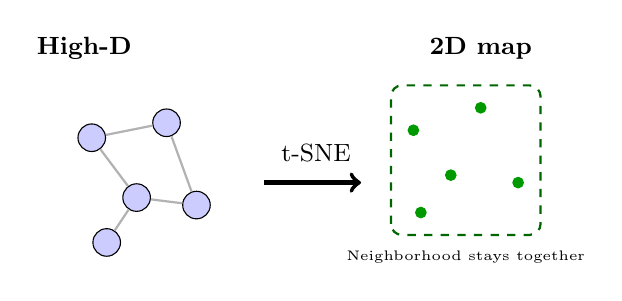
\begin{tikzpicture}[scale=0.95]
    % Left: high-D as a "neighborhood graph"
    \node[font=\small\bfseries] at (-0.1,3.2) {High-D};
    \foreach \p/\x/\y in {a/0/2, b/1/2.2, c/0.6/1.2, d/1.4/1.1, e/0.2/0.6} {
        \node[circle, draw, fill=blue!20, minimum size=0.35cm] (\p) at (\x,\y) {};
    }
    \draw[thick, gray!60] (a)--(b);
    \draw[thick, gray!60] (a)--(c);
    \draw[thick, gray!60] (c)--(d);
    \draw[thick, gray!60] (c)--(e);
    \draw[thick, gray!60] (b)--(d);

    % Arrow
    \draw[->, ultra thick] (2.3,1.4) -- (3.6,1.4);
    \node[font=\small] at (3.0,1.8) {t-SNE};

    % Right: 2D
    \node[font=\small\bfseries] at (5.2,3.2) {2D map};
    \foreach \x/\y in {4.3/2.1, 5.2/2.4, 4.8/1.5, 5.7/1.4, 4.4/1.0} {
        \filldraw[green!60!black] (\x,\y) circle (2pt);
    }
    \draw[rounded corners, dashed, thick, green!40!black] (4.0,0.7) rectangle (6.0,2.7);
    \node[font=\tiny, align=center] at (5.0,0.4) {Neighborhood stays together};
\end{tikzpicture}
\end{column}
\end{columns}

\end{frame}


% --- SLIDE: Example (synthetic PCA-like vs t-SNE-like) ---
\begin{frame}{Example: Visualizing MNIST via t-SNE}
\begin{figure}
    \centering
    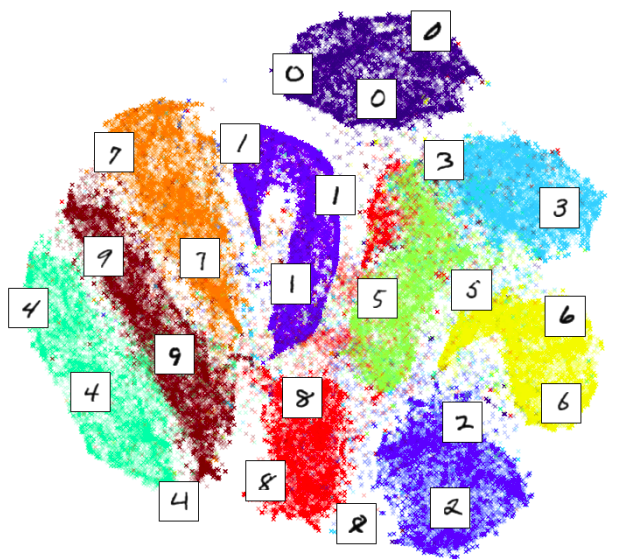
\includegraphics[width=0.4\linewidth]{images/tsne.png}
\end{figure}
\vspace{0.4em}
\centering
\small \textit{This is much better than PCA! We can see how similar digits are grouped together, while different ones are far from each other.}

\end{frame}








% --- SLIDE: Transition to Autoencoders ---
\begin{frame}[c]
\centering

We have covered classical algorithms like K-Means and PCA.

Now, let's explore a powerful Neural Network architecture designed for unsupervised learning...


\end{frame}


\section{Autoencoders}

% --- SLIDE 2: What is an Autoencoder? ---
